\documentclass[11pt,a4paper]{article}
\usepackage[margin=1in]{geometry}
\usepackage{amsmath,amssymb,amsthm}
\usepackage{hyperref}
\usepackage{setspace}
\usepackage{graphicx}
\usepackage{enumitem}
\usepackage{tikz}
\usepackage{xcolor}
\usepackage{booktabs}
\usepackage{caption}
\usepackage{subcaption}

% TikZ libraries for architecture diagram
\usetikzlibrary{shapes.geometric, arrows.meta, positioning, fit, backgrounds, calc, shadows.blur}

% Define colors for architecture diagram
\definecolor{inputcolor}{RGB}{65, 105, 225}
\definecolor{encodercolor}{RGB}{50, 205, 50}
\definecolor{attentioncolor}{RGB}{255, 165, 0}
\definecolor{outputcolor}{RGB}{220, 20, 60}
\definecolor{flowcolor}{RGB}{100, 100, 100}
\definecolor{bglight}{RGB}{245, 248, 255}

% Hyperref setup
\hypersetup{
    colorlinks=true,
    linkcolor=blue!70!black,
    citecolor=green!50!black,
    urlcolor=blue!70!black
}

\title{\textbf{Quaternion Neural Networks with Temporal Attention\\for Financial Time-Series Forecasting}}
\author{}
\date{}

\begin{document}
\maketitle
\onehalfspacing

\begin{abstract}
\noindent This thesis investigates the application of Quaternion Neural Networks (QNNs) augmented with temporal attention mechanisms for financial time-series forecasting. Financial markets exhibit complex multivariate dependencies that traditional real-valued neural networks may inadequately capture. By encoding Open, High, Low, and Close (OHLC) price data as quaternion-valued inputs, the proposed architecture exploits the algebraic structure of hypercomplex numbers to model inter-feature correlations more efficiently. A hybrid design combining quaternion-valued encoders with real-valued temporal attention enables the model to simultaneously capture feature dependencies and identify salient temporal patterns. Empirical evaluation on S\&P 500 data demonstrates the efficacy of this approach in terms of directional accuracy and prediction error metrics.
\end{abstract}

\section{Introduction}
\label{sec:introduction}

Financial time-series forecasting represents a fundamental challenge in quantitative finance, with applications spanning algorithmic trading, risk management, and portfolio optimization. The inherent characteristics of financial data---including non-stationarity, heavy-tailed distributions, and complex inter-asset dependencies---necessitate sophisticated modeling approaches capable of capturing subtle patterns within noisy observations.

Recent advances in deep learning have yielded substantial improvements in sequence modeling tasks, with recurrent architectures such as Long Short-Term Memory (LSTM) networks demonstrating particular efficacy in temporal prediction problems. However, conventional real-valued neural networks process input features independently, potentially overlooking structural relationships inherent in multivariate financial data.

This thesis proposes a novel architecture that addresses these limitations through two complementary mechanisms: (i) quaternion-valued neural network layers that encode related financial features as unified hypercomplex entities, and (ii) temporal attention mechanisms that adaptively weight historical observations based on their predictive relevance.

\subsection{Research Objectives}

The primary objectives of this research are:
\begin{enumerate}[noitemsep]
    \item To develop a hybrid quaternion-attention architecture tailored for financial time-series prediction
    \item To empirically evaluate the benefits of quaternion representations compared to real-valued alternatives
    \item To analyze the interpretability of learned attention weights in financial contexts
    \item To assess model robustness across different temporal granularities and market conditions
\end{enumerate}

\section{Theoretical Background}
\label{sec:background}

\subsection{Quaternion Algebra}

Quaternions, denoted $\mathbb{H}$, constitute a four-dimensional extension of complex numbers, first described by Hamilton in 1843. A quaternion $q \in \mathbb{H}$ is expressed as:
\begin{equation}
    q = w + xi + yj + zk
\end{equation}
where $w, x, y, z \in \mathbb{R}$ and $i, j, k$ are imaginary units satisfying:
\begin{equation}
    i^2 = j^2 = k^2 = ijk = -1
\end{equation}

The Hamilton product of two quaternions $q_1 = w_1 + x_1i + y_1j + z_1k$ and $q_2 = w_2 + x_2i + y_2j + z_2k$ is defined as:
\begin{equation}
    q_1 \otimes q_2 = (w_1w_2 - x_1x_2 - y_1y_2 - z_1z_2) + \ldots
\end{equation}

This non-commutative multiplication enables quaternion neural networks to learn rich interactions between the four components of each input.

\subsection{Quaternion Neural Networks}

Quaternion Neural Networks (QNNs) extend conventional neural architectures to operate in quaternion space. A quaternion linear transformation applies a quaternion weight $W = W_w + W_xi + W_yj + W_zk$ to a quaternion input $q$ via the Hamilton product:
\begin{equation}
    \text{output} = W \otimes q + b
\end{equation}

This formulation reduces the parameter count by approximately 75\% compared to equivalent real-valued transformations while enforcing structured interactions between input components.

\section{Problem Formulation}
\label{sec:problem}

The objective of this thesis is to investigate whether Quaternion Neural Networks combined with temporal attention mechanisms yield improved financial time-series predictions compared to traditional real-valued architectures.

Given a sequence of historical market observations $\{x_1, x_2, \ldots, x_T\}$, the task is to predict the asset price at the subsequent time step $\hat{y}_{T+1}$. While the model is trained in a regression setting, evaluation emphasizes \textbf{directional accuracy} (predicting whether price moves up or down), which provides a more robust assessment in noisy financial environments where exact price prediction is inherently uncertain.

\section{Methodology}
\label{sec:methodology}

\subsection{Data Representation}

At each time step $t$, market data are encoded as a quaternion:
\begin{equation}
    q_t = \text{Open}_t + \text{High}_t \cdot i + \text{Low}_t \cdot j + \text{Close}_t \cdot k
    \label{eq:quaternion_encoding}
\end{equation}

This representation treats OHLC prices as components of a single structured entity, enabling quaternion-valued layers to model their internal relationships through the Hamilton product. The encoding preserves the inherent structure of candlestick data, where all four components describe different aspects of the same trading period.

\subsection{Model Architecture}
\label{subsec:architecture}

The proposed architecture follows a hybrid encoder-attention design, illustrated in Figure~\ref{fig:architecture}. The model comprises four principal components: (i) a quaternion input embedding layer, (ii) a quaternion LSTM encoder, (iii) a real-valued temporal attention mechanism, and (iv) a prediction head.

\begin{figure}[htbp]
\centering
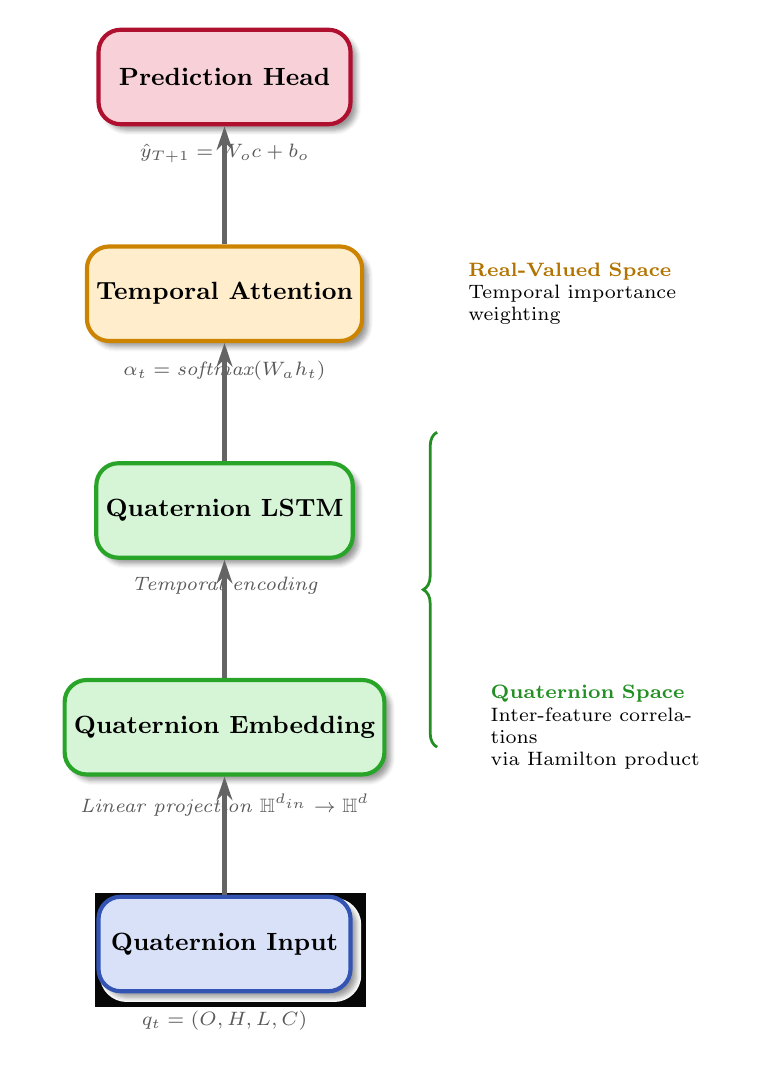
\begin{tikzpicture}[
    node distance=0.8cm and 1.5cm,
    >={Stealth[length=3mm, width=2mm]},
    % Node styles
    inputnode/.style={
        rectangle,
        rounded corners=8pt,
        minimum width=3.2cm,
        minimum height=1.2cm,
        text centered,
        draw=inputcolor!80!black,
        fill=inputcolor!20,
        line width=1.5pt,
        font=\small\bfseries,
        blur shadow={shadow blur steps=5, shadow xshift=0.5ex, shadow yshift=-0.5ex}
    },
    encodernode/.style={
        rectangle,
        rounded corners=8pt,
        minimum width=3.2cm,
        minimum height=1.2cm,
        text centered,
        draw=encodercolor!80!black,
        fill=encodercolor!20,
        line width=1.5pt,
        font=\small\bfseries,
        blur shadow={shadow blur steps=5, shadow xshift=0.5ex, shadow yshift=-0.5ex}
    },
    attentionnode/.style={
        rectangle,
        rounded corners=8pt,
        minimum width=3.2cm,
        minimum height=1.2cm,
        text centered,
        draw=attentioncolor!80!black,
        fill=attentioncolor!20,
        line width=1.5pt,
        font=\small\bfseries,
        blur shadow={shadow blur steps=5, shadow xshift=0.5ex, shadow yshift=-0.5ex}
    },
    outputnode/.style={
        rectangle,
        rounded corners=8pt,
        minimum width=3.2cm,
        minimum height=1.2cm,
        text centered,
        draw=outputcolor!80!black,
        fill=outputcolor!20,
        line width=1.5pt,
        font=\small\bfseries,
        blur shadow={shadow blur steps=5, shadow xshift=0.5ex, shadow yshift=-0.5ex}
    },
    arrow/.style={
        ->,
        line width=1.5pt,
        color=flowcolor
    },
    sublabel/.style={
        font=\scriptsize\itshape,
        text=gray!70!black
    }
]

% Background
\begin{scope}[on background layer]
    \fill[bglight, rounded corners=15pt] (-2.5,-0.8) rectangle (2.5,10.8);
\end{scope}

% Nodes
\node[inputnode] (input) {Quaternion Input};
\node[sublabel, below=0.1cm of input] (inputsub) {$q_t = (O, H, L, C)$};

\node[encodernode, above=1.5cm of input] (embed) {Quaternion Embedding};
\node[sublabel, below=0.1cm of embed] (embedsub) {Linear projection $\mathbb{H}^{d_{in}} \to \mathbb{H}^{d}$};

\node[encodernode, above=1.5cm of embed] (lstm) {Quaternion LSTM};
\node[sublabel, below=0.1cm of lstm] (lstmsub) {Temporal encoding};

\node[attentionnode, above=1.5cm of lstm] (attention) {Temporal Attention};
\node[sublabel, below=0.1cm of attention] (attsub) {$\alpha_t = \text{softmax}(W_a h_t)$};

\node[outputnode, above=1.5cm of attention] (output) {Prediction Head};
\node[sublabel, below=0.1cm of output] (outsub) {$\hat{y}_{T+1} = W_o c + b_o$};

% Arrows
\draw[arrow] (input) -- (embed);
\draw[arrow] (embed) -- (lstm);
\draw[arrow] (lstm) -- (attention);
\draw[arrow] (attention) -- (output);

% Side annotations
\node[right=1.2cm of embed, text width=3cm, font=\scriptsize, align=left] (ann1) {
    \textcolor{encodercolor!70!black}{\textbf{Quaternion Space}}\\
    Inter-feature correlations\\
    via Hamilton product
};

\node[right=1.2cm of attention, text width=3cm, font=\scriptsize, align=left] (ann2) {
    \textcolor{attentioncolor!70!black}{\textbf{Real-Valued Space}}\\
    Temporal importance\\
    weighting
};

% Decorative brackets
\draw[decorate, decoration={brace, amplitude=5pt}, encodercolor!70!black, line width=1pt]
    (2.7,2.5) -- (2.7,6.5) node[midway, right=8pt, font=\scriptsize\bfseries, text=encodercolor!70!black] {};

\end{tikzpicture}
\caption{Architecture of the proposed Quaternion-Attention model for financial time-series forecasting. The model processes quaternion-encoded OHLC data through a quaternion embedding layer and LSTM encoder (operating in quaternion space), followed by a real-valued temporal attention mechanism that computes context-aware predictions.}
\label{fig:architecture}
\end{figure}

\subsubsection{Quaternion Embedding Layer}

The input quaternion sequence $\{q_1, q_2, \ldots, q_T\}$ is first projected through a quaternion linear layer:
\begin{equation}
    h_t^{(0)} = W_e \otimes q_t + b_e
\end{equation}
where $W_e \in \mathbb{H}^{d_{in} \times d}$ and $b_e \in \mathbb{H}^d$ are learnable quaternion parameters.

\subsubsection{Quaternion LSTM Encoder}

The embedded sequence is processed by a Quaternion LSTM, which extends the standard LSTM formulation to quaternion space. The quaternion LSTM maintains quaternion-valued hidden states $h_t \in \mathbb{H}^d$ and cell states $c_t \in \mathbb{H}^d$, with gates computed via quaternion operations:
\begin{align}
    f_t &= \sigma(W_f \otimes [h_{t-1}, q_t] + b_f) \\
    i_t &= \sigma(W_i \otimes [h_{t-1}, q_t] + b_i) \\
    o_t &= \sigma(W_o \otimes [h_{t-1}, q_t] + b_o) \\
    \tilde{c}_t &= \tanh(W_c \otimes [h_{t-1}, q_t] + b_c) \\
    c_t &= f_t \odot c_{t-1} + i_t \odot \tilde{c}_t \\
    h_t &= o_t \odot \tanh(c_t)
\end{align}

This formulation captures both inter-feature dependencies (through quaternion multiplications) and temporal dynamics (through the recurrent structure).

\subsubsection{Temporal Attention Mechanism}

A real-valued attention mechanism is applied to the sequence of hidden states $\{h_1, h_2, \ldots, h_T\}$ to compute a context vector. First, the quaternion hidden states are converted to real-valued representations by concatenating their four components. Attention weights are then computed as:
\begin{equation}
    \alpha_t = \frac{\exp(W_a \cdot \text{real}(h_t))}{\sum_{t'=1}^{T} \exp(W_a \cdot \text{real}(h_{t'}))}
\end{equation}

The context vector is obtained as:
\begin{equation}
    c = \sum_{t=1}^{T} \alpha_t \cdot \text{real}(h_t)
\end{equation}

\subsubsection{Prediction Head}

The final prediction is computed through a fully connected layer:
\begin{equation}
    \hat{y}_{T+1} = W_p \cdot c + b_p
\end{equation}

\subsection{Design Rationale}

The hybrid architecture deliberately separates two modeling concerns: (i) \textit{feature correlation modeling} in quaternion space, where the Hamilton product naturally captures interactions between OHLC components, and (ii) \textit{temporal importance modeling} in real-valued space, which maintains computational efficiency and interpretability. Full quaternion-valued attention would introduce additional complexity without clear theoretical justification for temporal weighting in hypercomplex space.

\section{Experimental Design}
\label{sec:experiments}

\subsection{Dataset}

Experiments are conducted on S\&P 500 index data and selected constituent stocks. Publicly available OHLC price data are obtained from Yahoo Finance, with hourly resolution as the primary time scale and daily data for robustness analysis.

\subsection{Baseline Models}

The proposed architecture is compared against:
\begin{itemize}[noitemsep]
    \item \textbf{Real-valued LSTM}: Standard LSTM with concatenated OHLC features
    \item \textbf{Quaternion LSTM}: Quaternion encoder without attention mechanism
    \item \textbf{Real-valued LSTM with Attention}: Standard attention-augmented LSTM
\end{itemize}

\subsection{Evaluation Metrics}

Model performance is assessed using:
\begin{itemize}[noitemsep]
    \item \textbf{Directional Accuracy}: Percentage of correct up/down predictions
    \item \textbf{Mean Absolute Error (MAE)}: Average absolute prediction error
    \item \textbf{Mean Squared Error (MSE)}: Average squared prediction error
    \item \textbf{Sharpe Ratio}: Risk-adjusted returns in simulated trading scenarios
\end{itemize}

\subsection{Validation Strategy}

Rolling window cross-validation is employed to respect temporal ordering and prevent look-ahead bias. The training window expands incrementally while maintaining a fixed validation horizon.

\section{Implementation}
\label{sec:implementation}

The model is implemented in Python using the PyTorch deep learning framework. Quaternion operations are built upon existing open-source implementations, extended with finance-specific preprocessing and evaluation modules. All experiments are conducted with fixed random seeds to ensure reproducibility.

\section{Expected Contributions}
\label{sec:contributions}

The anticipated contributions of this thesis include:
\begin{enumerate}[noitemsep]
    \item A novel hybrid architecture combining quaternion neural networks with temporal attention for financial forecasting
    \item Empirical evidence regarding the efficacy of quaternion representations for modeling OHLC price data
    \item Analysis of attention weight interpretability in financial prediction contexts
    \item Practical insights into the application of hypercomplex neural networks in quantitative finance
\end{enumerate}

\section{Conclusion}
\label{sec:conclusion}

This thesis proposes a principled approach to financial time-series modeling that leverages the algebraic structure of quaternions to encode multivariate market data. By combining quaternion-valued neural network layers with temporal attention mechanisms, the proposed architecture aims to capture both inter-feature dependencies and salient temporal patterns. Empirical evaluation on S\&P 500 data will assess whether this structured representation provides measurable advantages over conventional real-valued approaches in noisy financial environments.

\end{document}
